%% Introduction
\section{Introduction}
\lettrine[lines=2]{A}{ctive} Noise Control (ANC) is a used method in a wide variety of applications. Research is being done in creating silents zones\cite{SilentZones}, improving room acoustics using multiple loudspeakers\cite{CAPS} and is already available in various headphones.
% for noise cancellation, both for professional and consumer use. 

Noise canceling headphones are used in various environments which have different noise characteristics. These characteristics vary from periodic low frequency noise (10-200 Hz), e.g. from machinery and helicopter rotor\cite{LowFrequency}, mid-range frequency noise (200-4000 Hz), e.g. speech \cite{MidFrequency}, to high frequency noise (4-20 kHz), e.g. turbine noise \cite{LowFrequency}. The high frequency noise is naturally attenuated by using a closed headphone cup \cite{naturalAttenuation} and static low frequency noise are attenuated by the present consumer headphones \cite{naturalAttenuation}.Speech can be shown in figure \ref{fig:ANCcompare}, not to be attenuated by active noise cancellation in present market ANC headphones.
%\footnote{Numbers and sources will be added to the statements}.   
%%ANC are used by companies such as Bang \& Olufsen and Lyngdorf Audio in their proprietary technology as Active Room Compensation\texttrademark and RoomPerfect\texttrademark respectively, to control noise in a room using loudspeakers. Headphone industries have adapted it into cancellation of noise and is used 

\begin{figure}[H]
	\centering
	\textbf{\textit{Here is going to be a graph of different}}
	\textbf{\textit{ headphones tested with non stationary signals (Speech)}}
	\caption{It is clearly seen that speech is not attenuated by current headphones.}
	\label{fig:ANCcompare}
\end{figure}


This paper will be focusing on attenuation of speech using an ANC-system. Speech will hence be seen as the primary noise source. The solution will be based on a digital feedforward system using the Filtered-X Least Mean Squares (FXLMS). The solution is chosen due to it being the optimal system for non stationary signals \cite{Hansen2}. The general solutions in ANC are described thoroughly by Hansen et al. \cite{Hansen}.

The problem of a feedforward system, shown in figure \ref{fig:SystemOverview}, is the dependency of noise having a larger propagation delay from the noise is measured (1) to a headphone loudspeaker(2) can produce a counter-phase signal in the desired point(3). 

{
	\centering
	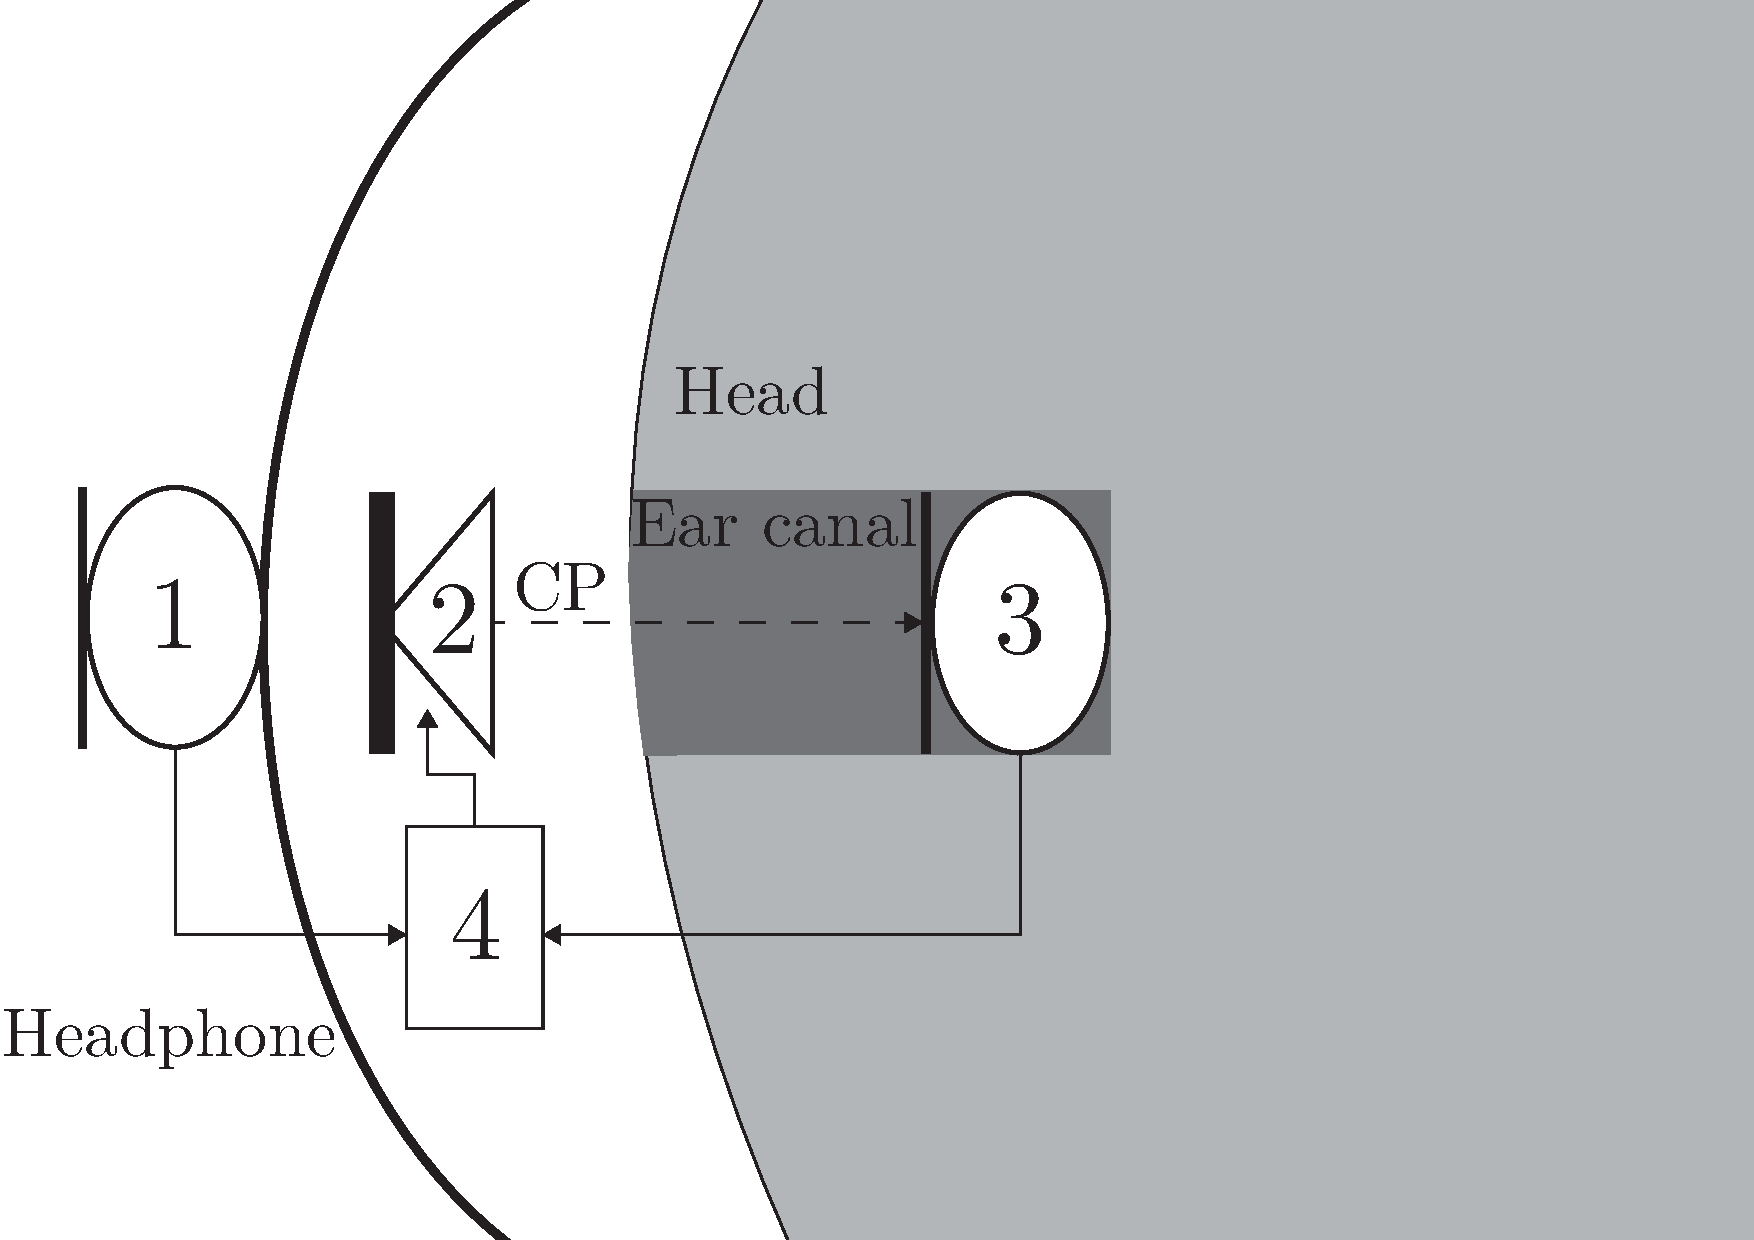
\includegraphics[width=1\columnwidth]{figures/ArticleIllustrations/BasicOverviewZoomed}
	\captionof{figure}{Simplified circumaural ANC Headphone fitted on ear. Showing the reference microphone (1), a headphone loudspeaker (2), an error microphone (3) and a DSP (4).}
	\label{fig:SystemOverview}
}

When implemented in a real-time system delay will occur, introduced by sampling and processing of the signal. For instance, measured on a cost-wise $\Sigma\Delta$ -converter\footnote{TLV320AIC3204} a sampling/conversion delay in the range of 220 $\mu$s to 880 $\mu$s is introduced, depending on a sampling frequency of 192 kHz to 48 kHz respectively. Assuming a $\text{0}^{\circ}$ angle of incident, which is the ideal case, the reference microphone must be placed 75.5 mm to 302 mm further out from the error microphone, to compensate for the delay. Instead a Linear Prediction (LP) scheme is proposed as a solution. In speech encoding Wiener filtering is often used therefore the Wiener filtering is the choosen prediction method \cite{Speech}.
% This reduces computation time and overall
%Consumer ANC headphones has a bandwidth that does not cover the entire frequency area of speech. This paper examines how to extend the bandwidth.
%To increase bandwidth a prediction algorithm is proposed as a potential solution. 
Prediction of speech is described by Wai C. Chu \cite{Speech}. 
%In this paper we will combine the reference solution with the prediction of speech to increase the bandwidth of a real time system.  

%The paper is split into two parts. The first part describes the feedforward FXLMS system and how to predict speech using linear prediction. The second part describes simulations and the implementation. Performance of the feedforward FXLMS system with and without prediction are determined and compared.

This paper firstly presents the feedforward FXLMS system and prediction by Wiener filtering, secondly presents the results of the proposed solution, thirdly discusses the results and lastly concludes on the proposed solution.
        
%why performance decreases with increased frequency and



%  The scope of this paper is not to derive a new ANC algorithm, but rather to expand the existing FXLMS algorithm by prediction. The goal of this modification is to achieve increased performanec, especially at higher frequencies.\\
% The application of the system is cancellation of speech in a call centre. The choice of a specific use case allows the frequency range and signal type of interest to be defined before designing the system. Call centres is an especially interesting environment for an ANC system, because the unwanted noise and the wanted signal have the same  characteristics as they are both speech. \\
% The paper is split into three parts. The first part examines the demands for an ANC system to be used in a call centre. The second part discus the algorithm used and shows preliminary results from simulations. The third part describes the real time implementation of the algorithm and verifies the performance of the ANC system.  




% \lettrine[lines=2]{A}{ctive} Noise Control (ANC) is a field of study, where a lot of algorithms are already known. The scope of this paper is not to derive a new ANC algorithm, but rather to expand the existing FXLMS algorithm by prediction. The goal of this modification is to achieve increased performanec, especially at higher frequencies.\\
% The application of the system is cancellation of speech in a call centre. The choice of a specific use case allows the frequency range and signal type of interest to be defined before designing the system. Call centres is an especially interesting environment for an ANC system, because the unwanted noise and the wanted signal have the same  characteristics as they are both speech. \\
% The paper is split into three parts. The first part examines the demands for an ANC system to be used in a call centre. The second part discus the algorithm used and shows preliminary results from simulations. The third part describes the real time implementation of the algorithm and verifies the performance of the ANC system.  




%\lettrine[lines=2]{A}{ctive} Noise Control (ANC) is a field of study, where a lot of algorithms are already known. \todo[inline]{$MENTION A FEW$} The scope of this paper is not to derive a new ANC algorithm, but rather to use an existing algorithm in a practical application. The application is cancellation of speech in a call centre The choice of a specific use case allows the frequency range and signal type of interest to be defined before designing the system. Call centres is an especially interesting environment for an ANC system, because the unwanted noise and the wanted signal have the same  characteristics as they are both speech. \\
%The paper is split into three parts. The first part examines the demands for an ANC system to be used in a call centre. The second part discus the algorithm used and shows preliminary results from simulations. The third part describes the real time implementation of the algorithm and verifies the performance of the ANC system.  